\section{Introduction}
\label{sec:intro}
The Cariban language family is one of the largest of South America, with between 60'000 and 100'000 speakers unevenly distributed between 22 to 25 extant languages \parencite[441]{gildea2012classification}.
The family is concentrated in Venezuela, the Guianas and Northern Brazil, with two Western and four Southern outliers.
\cref{fig:phylomap} gives an overview of the geographical distribution and genealogical affiliation of the extant Cariban languages.
%Cariban languages feature relatively rich verbal morphology, both pre- and suffixes, inflecting for person, number, tense, aspect, and evidentiality, combined with a range of valency-modifying affixes.
%Many also have a split-\gl{s} system, which can be reconstructed to \PC \pcref{sec:split}.
For linguistic overviews of and large-scale comparative work on the family, readers are referred to \textcites{gildea1998}{derbyshire1999carib}{meira2002first}{meira2005southern}{meira2006cariban}{gildea2007greenberg}{meira2010origin}{gildea2010story}{gildea2012classification}{matter2021cariban}{gildea2019overview}.

\begin{figure}
	\centering
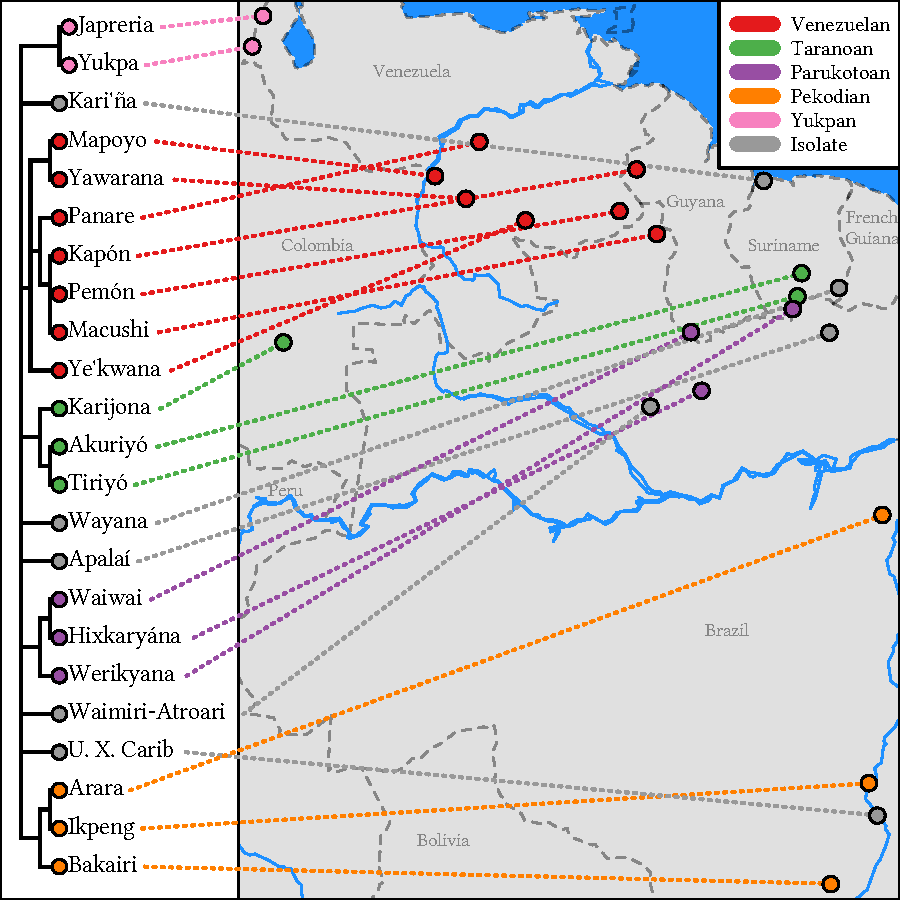
\includegraphics{floats/genealogical_map}
	\caption{The Cariban language family}
	\label{fig:phylomap}
\end{figure}

\begin{table}[htbp]
\centering
\caption[Some \hixka verbs]{Some \hixka verbs \parencites[150, 510, 511, 513, 520]{howard2001wrought}[197, 198]{hixkaryanaderby1985}}
\label{tab:hixintro}
\begin{tabular}[t]{@{}llllll@{}}
\mytoprule
{} &     \qu{to fall} &  \qu{to be afraid} &          \qu{to walk} & \qu{to cut self} &    \qu{to be} \\
\mymidrule
\gl{1}   &  \obj{k-ehurka-} &  \obj{k-oserʲehɨ-} &  \obj{k-atarʲeknohɨ-} &   \obj{k-atama-} &  \obj{w-eʃe-} \\
\gl{2}   &  \obj{m-ehurka-} &  \obj{m-oserʲehɨ-} &  \obj{m-atarʲeknohɨ-} &   \obj{m-atama-} &  \obj{m-eʃe-} \\
\gl{1+2} &  \obj{t-ehurka-} &  \obj{t-oserʲehɨ-} &  \obj{t-atarʲeknohɨ-} &   \obj{t-atama-} &  \obj{t-eʃe-} \\
\gl{3}   &  \obj{ɲ-ehurka-} &  \obj{n-oserʲehɨ-} &  \obj{n-atarʲeknohɨ-} &   \obj{n-atama-} &  \obj{n-eʃe-} \\
\mybottomrule
\end{tabular}
\end{table}
\begin{table}
\centering
\caption[Some \trio verbs]{Some \trio verbs \parencites[292, 294]{triomeira1999}[274]{triocarlin2004}}
\label{tab:triintro}
\begin{tabular}[t]{@{}llllll@{}}
\mytoprule
{} &      \qu{to sleep} & \qu{to see self} & \qu{to bathe (\gl{intr})} &     \qu{to yawn} &     \qu{to go} \\
\midrule
\gl{1}   &    \obj{t-əənɨkɨ-} &    \obj{t-əene-} &              \obj{s-epɨ-} &  \obj{s-entapo-} &  \obj{wɨ-tən-} \\
\gl{2}   &    \obj{m-əənɨkɨ-} &    \obj{m-əene-} &              \obj{m-epɨ-} &  \obj{m-entapo-} &  \obj{mɨ-tən-} \\
\gl{1+2} &  \obj{kɨt-əənɨkɨ-} &    \obj{k-əene-} &             \obj{ke-epɨ-} &  \obj{k-entapo-} &  \obj{kɨ-tən-} \\
\gl{3}   &    \obj{n-əənɨkɨ-} &    \obj{n-əene-} &              \obj{n-epɨ-} &  \obj{n-entapo-} &  \obj{nɨ-tən-} \\
\bottomrule
\end{tabular}
\end{table}

Some Cariban languages show a small group of verbs which diverge in their first person inflection pattern.
This is illustrated for \hixka in \cref{tab:hixintro},\footnote{The presence of a \gl{1+2} person value implies that of a \gl{1+3} value.
This is usually expressed with a free pronoun combined with third person morphology in Cariban languages, so it is not represented as a distinct value in the paradigms shown here.
In \cref{tab:hixintro} and other paradigm tables, any TAM suffixes found in the original forms found in the literature are omitted, since a) the focus lies on the prefixes and stems, and b) full paradigms containing the same TAM suffix are rarely found.
Further, standard IPA symbols are used in the transcription of Cariban languages, with the exception of coronal rhotics, which are simply represented with \ort{r}, rather than \ort{ɽ} for \wayana or \ort{ɾ̠} for \maqui etc.
In languages with strong morphophonological processes and/or subphonemic orthography the original transcription is shown in an additional surface line when presented in interlinearized examples.
\textcite{gildea2018reconstructing} is followed in using \ort{ə} for the proto-vowel reconstructed by \textcite{meira2005southern}, although it was likely more back \parencite{gildea2010story}.
Glossing abbreviations: }%\glossingAbbrevsComma.
which shows person paradigms for four verbs, all members of the \gl{s_a_} inflectional class.
In this language, the verb \qu{to be} diverges in its first person marker (\obj{w-}), contrasting with other \gl{s_a_} verbs like \qu{to fall}, which have \obj{k(ɨ)-}.
A similar pattern can be found in \trio, where the verb \qu{to go} has a first-person prefix \obj{wɨ-} while other \gl{s_a_} verbs have a prefix with phonologically conditioned allomorphs \envr{\obj{t-}}{\obj{ə}} and \envr{\obj{s-}}{\obj{e}} \pcref{tab:triintro}.
In both languages, the inflectional patterns of the verbs on the left of the table is representative for the vast majority of \gl{s_a_} verbs.
%In both languages, there are only a few other verbs inflected identically to the divergent ones on the right; for example, the first-person form of \trio \qu{to be} is \obj{w-ei-} \parencites[339]{triomeira1999}.

In the literature, such divergent verbs have been identified for \hixka \parencite[188]{hixkaryanaderby1985}, \waiwai \parencite[90]{gildea1998}, the three Taranoan languages \parencite[112--115]{meira1998proto}, \bakairi \parencite{meira2003bakairi}, and \arara \parencite[153]{alves2017arara}.
In a language-specific synchronic analysis, these verbs and their first person prefixes may be considered to be \textsc{irregular}, contrasting with regular prefixes, like \hixka \obj{k(ɨ)-} and \trio \obj{t-}/\obj{s-}, on regular verbs.
However, there is no widely accepted definition of irregularity \parencite{stolz2012introduction}, and many stricter definitions \parencite[][e.g.]{haspelmath2010understanding} require the pattern to occur at a single place in the grammar.
For such approaches, these verbs simply belong to a small inflectional (sub-)class, an analysis found in the literature for the Pekodian languages \bakairi and \arara \parencites[4]{meira2003bakairi}[149]{alves2017arara}.

Regardless of the synchronic analysis, the reason for these inflectional patterns can be found in the diachrony of the languages in question.
The purpose of this paper is to approach the patterns from a comparative perspective and to provide a unifying diachronic account, proceeding as follows.
In \cref{sec:background}, readers are provided with necessary background knowledge about \PC verbs, and the mechanism of person marker extensions is introduced.
In \cref{sec:data}, six incomplete person marker extensions and their extent in the lexicon are described.
Since there is a surprising amount of agreement about what verbs remain conservative, they are compared and reconstructed.
\cref{sec:motivations} uses \posscite{bybee1985morphology} network model of morphology to find explanations for the verbs (not) affected by each extension.
\cref{sec:discussion} summarizes and discusses the results, and puts them in a general context of language change.

% analyses:
%\begin{inlinelist}
%	\item special copula prefix \parencite[188]{hixkaryanaderby1985}
%	\item inflectional subclass \parencites[149]{alves2017arara}[4]{meira2003bakairi}
%	\item \dbqu{exceptional cases} \parencite[293]{triomeira1999}
%	\item phonologically conditioned allomorphs \parencites[139]{meira2006syntactic}{meira2003primeras}[189]{hixkaryanaderby1985}
%	\item not discussed \parencites{waiwaihawkins1998}{ikpengpacheco2001}{alves2013verbo}{pacheco2003intransitivos}
%\end{inlinelist}.
%meira: non-detransitivized verbs
%alves: non-detransitivized verbs (as a consequence, o-initial)